\documentclass[../main.tex]{subfiles}
\begin{document}
Write a java program to simulate a traffic light. The program lets the user
select one of the three lights: red, yellow, or green. On selecting a button,
an appropriate message with ”Stop”, “Ready” or “ Go” should appear above the
buttons selected color.

\subsection{Code}
\inputminted[frame=lines, breaklines, breakanywhere, numberblanklines=false]{java}{./programs/prog13/Traffic.java}

\subsection{Output}
\begin{figure}[h!]
	\centering
	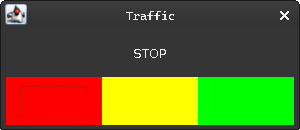
\includegraphics[width=0.3\textwidth]{./assets/p13-s1.png}
	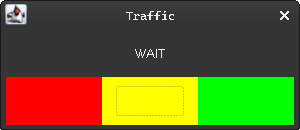
\includegraphics[width=0.3\textwidth]{./assets/p13-s2.png}
	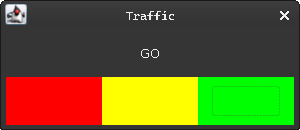
\includegraphics[width=0.3\textwidth]{./assets/p13-s3.png}
\end{figure}

\end{document}
